\chapter{Цел}

\section{Въведение}
Неперовото число е една от най-значимите константи в математиката и инженерните науки \cite{wiki-napier}. В този проект ще разгледаме един от възможните начини за пресмятане на неперовото число, използвайки сумиране на ред. Този начин за пресмятане е особено удобен, защото позволява много лесно паралелизиране на изчислението. Проектът се състои във създаването на програма на Java, която може да бъде изпълнена от командния ред.

\section{Ускорение}
Целта ни е да намерим как се мени времето за изпълнение според броя нишки, които използваме при паралелното сумиране. За целта програмата може да бъде изпълнена в два режима - за изчисление и за сравнение. В режим "изчисление" даваме на програмата прецизността (колко члена на реда искаме да съберем), колко нишки да използваме, файл, в който да запишем резултата. В режим "сравнение" даваме прециозност, максимален брой нишки и файл, в който да се запишат резултатите за различният брой нишки. В режим "сравнение" просто се изпълнява същото, както в режим "изчисление", но с различен брой нишки - вариращ от 1 до дадения максимален брой.


\chapter{Алгоритъм и изпълнение}

\section{Ред}
Редът, който ще използваме за пресмятането на неперовото число, е следният:

\[ e = \sum_{k = 0}^{\infty} \frac{2k + 1}{(2k!)} \]

Програмата ще разпредели членовете на сумата между нишките и след това ще сумира резултатите по тях. Например ако програма получи като вход броя членове да е 2000 и нишките да са 4, тя ще разпредели на нишка 0 да сумира от 0 до 500, на нишка 1 - от 500 до 1000, на нишка 2 - от 1000 до 1500 и на нишка 3 от 1500 до 2000, след което ще сумира резултатите от всяка от тях.


\section{Изпънение}

Ще сравним за фиксирана прецизност от 1000, 2000, 3000, 4000 и 5000 при различен брой нишки (от 1 до 32) как се мени скоростта на изчислението.

\chapter{Реализация}

\section{Имплементация}

Главният клас на програмата се казва App. В неговия main метод се парсват аргументите, подадени от командния ред чрез библиотеката Docopt и се извиква подходяща инстанция на интерфейса CommandHandler в зависимост от извиканата команда - BenchmarkCommandHandler или ComputeCommandHandler. Във ComputeCommandHandler инстанция на класа RunnablesScheduler разпределя интервалите, които всяка нишка трябва да сумира и връща списък от NapierComputation. Този клас представя сумиране на дадените членове за фиксиран интервал. След това този списък от NapierComputation инстанции се изпълнява чрез класа CompositeNapierComputation, който създава нишка за всеки NapierComputation и ги пуска паралелно. BenchmarkCommandHandler от своя страна просто итерира от 1 до максимания брой нишки като изпълнява същото като в ComputeCommandHandler и накрая записва резултата във файл. Резутатът представлява серия от редове, като всеки ред се състои от брой нишки и времето в милисекунди, което е отнело за изпълнение.

\section{Използвани класове и библиотеки}

Използваните класове от стандартната библиотека и външните библиотеки включват:

\begin{enumerate}
    \item Docopt - за парсване на аргументи от командния ред
    \item ExecutionService - за паралелно изпълнение на нишките
    \item Calendar - за засичане на времето
    \item BigDecimal - за прецизни операции с плаваща запетая.
\end{enumerate}

\section{Интерфейс от командния ред}
Програмата може да бъде изпълнена с аргумент -h или --help, при което се появява документацията: 

\begin{lstlisting}[language=bash, caption=Помощно съобщение]
napier.

    Usage:
        napier compute -p <precision> -t <tasks> -o <output> [-q]
        napier benchmark -p <precision> -t <tasks> -o <output> [-q]
        napier (-h | --help)
        napier --version

    Commands:
        compute                         Performs computation by 
                                        a given number of summation terms,
                                        maximum number of tasks and
                                        output file to dump to.
        benchmark                       For a given fixed precision, runs
                                        computation with tasks from 1 to the 
                                        given maximum number and dumps
                                        csv file with the results.

    Options:
        -h --help                       If present, help is shown.
        --version                       Show version.
        -p --precision <precision>      The number of summation terms in the 
                                        series approximation.
        -t --tasks <tasks>              The maximum number of tasks
        -o --output <output>            The output file. The result is dumped 
                                        to this file.
        -q --quiet                      If set to true, does not output
                                        information about thread starting 
                                        and stopping.

\end{lstlisting}

\chapter{Измервания и анализ}
Нека сега се спрем на измерванията в графичен и табличен вид. В случая сме фиксирали прецизност 5000, а останалите измервания, както и скриптове за генериране на таблиците и графиките, могат да бъдат намерени в хранилището на проекта \cite{github-repo}.

\section{Графика}

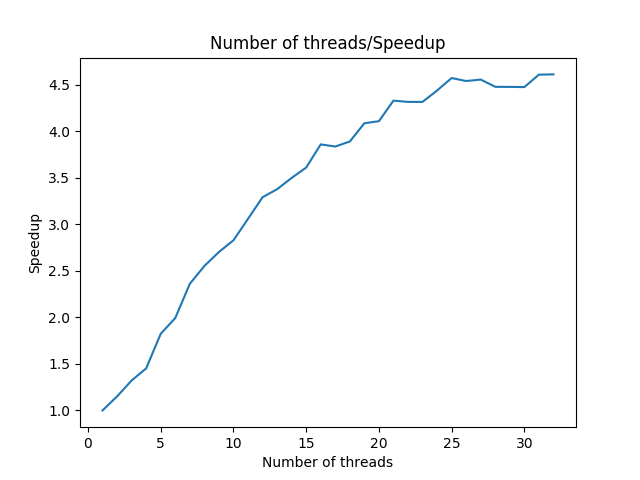
\includegraphics{speedup}

\section{Таблица}
Времето за изпълнението на серийната програма е $$T_1 = 79830$$

Таблицата с различния брой нишки и ускорението изглежда по следния начин:

\begin{center}
 \begin{tabular}{||c c c c||} 
 \hline
 Брой нишки & Време за изпънение в ms & Ускорение \\ [0.5ex] 
 \hline
		\hline
			1 & 79830.0 & 1.0 \\
		

		\hline
			2 & 69395.0 & 1.1503710641977087 \\
		

		\hline
			3 & 60394.0 & 1.3218200483491738 \\
		

		\hline
			4 & 54999.0 & 1.4514809360170184 \\
		

		\hline
			5 & 43771.0 & 1.8238102853487468 \\
		

		\hline
			6 & 40057.0 & 1.992910103103078 \\
		

		\hline
			7 & 33824.0 & 2.360158467360454 \\
		

		\hline
			8 & 31280.0 & 2.5521099744245523 \\
		

		\hline
			9 & 29543.0 & 2.7021629489219103 \\
		

		\hline
			10 & 28226.0 & 2.8282434634733935 \\
		

		\hline
			11 & 26101.0 & 3.0585035056128116 \\
		

		\hline
			12 & 24258.0 & 3.2908731140242393 \\
		

		\hline
			13 & 23639.0 & 3.3770464063623673 \\
		

		\hline
			14 & 22819.0 & 3.4984004557605504 \\
		

		\hline
			15 & 22115.0 & 3.609767126384807 \\
		

		\hline
			16 & 20687.0 & 3.858945231304684 \\
		

		\hline
			17 & 20812.0 & 3.835767826254084 \\
		

		\hline
			18 & 20522.0 & 3.889971737647403 \\
		

		\hline
			19 & 19538.0 & 4.0858839185177604 \\
		

		\hline
			20 & 19433.0 & 4.107960685431997 \\
		

		\hline
			21 & 18440.0 & 4.329175704989154 \\
		

		\hline
			22 & 18499.0 & 4.3153683982918 \\
		

		\hline
			23 & 18498.0 & 4.315601686668829 \\
		

		\hline
			24 & 17988.0 & 4.437958639092728 \\
		

		\hline
			25 & 17461.0 & 4.571903098333429 \\
		

		\hline
			26 & 17585.0 & 4.539664486778505 \\
		

		\hline
			27 & 17524.0 & 4.555466788404474 \\
		

		\hline
			28 & 17829.0 & 4.477536597677941 \\
		

		\hline
			29 & 17832.0 & 4.47678331090175 \\
		

		\hline
			30 & 17841.0 & 4.474524970573398 \\
		

		\hline
			31 & 17323.0 & 4.608324193269064 \\
		

		\hline
			32 & 17313.0 & 4.61098596430428 \\  [1ex] 
 \hline
\end{tabular}
\end{center}
 